%% Tex spellcheck
% Maybe put this as Chapter 2

% Write in English.
\chapter{Chapter 2 : Technical Concepts}

In this chapter, we will brifely explore different technical concepts that are important to understand the rest of the document. We will start by defining what a \gls{gnss} is, basic \gls{rf} concepts, trilateration and finally a brief introduction to \gls{sdr}.


\section{GNSS}

A \gls{gnss} is a satellite-based navigation system that provides location and time informations. These systems are used in a massive variety of domains around us and have been adopted by many industries including agriculture, aviation, construction, maritime, mining, public safety, transportation, etc.

Several \gls{gnss} have been developed\footcite{noauthor_satellite_2024} in different countries / regions and are in operation around the world, five of them being worldwide systems, thus available globally anywhere in the world:

\begin{itemize}
	\item United States's \textbf{\gls{gps}}
	\item Russia's \textbf{\gls{glonass}}
	\item European Union's \textbf{\gls{galileo}}
	\item China's \textbf{\gls{beidou}}
\end{itemize}

Two other systems are regional :
\begin{itemize}
	\item India's \textbf{\gls{irnss}}
	\item Japan's \textbf{\gls{qzss}}
\end{itemize}

% TODO: CITE THE CHAPTER ?
We won't go into details about every \gls{gnss} but only for GPS which is the most widely used and supported by the majority of devices.

\section{Radio Frequencies}

% Basic introduction to genaral Radio frequencies

Radio frequencies are a space within the electromagnetic spectrum associated with radio wave propagation. It is used to transmit information across distances. It's done by modulating the information on a carrier wave. The carrier wave is then transmitted through an antenna and received by another antenna. The information is then demodulated and the original information is recovered.

\subsection{Modulation}

Modulation is the process of varying one or more properties of a waveform (Amplitude, Phase, Frequency) in order to encode information or actual bits. The information is then carried by the carrier wave. The process of recovering the original information is called demodulation. We can vary one of the properties at the time or combine them to create more complex modulation schemes. The most common modulation schemes are:

\begin{itemize}
	\item \gls{am}
	\item \gls{fm}
	\item \gls{pm}
	\item \gls{bpsk}
	\item \gls{qpsk}
	\item \gls{qam}
\end{itemize}


\begin{figure}[H]
	\centering
	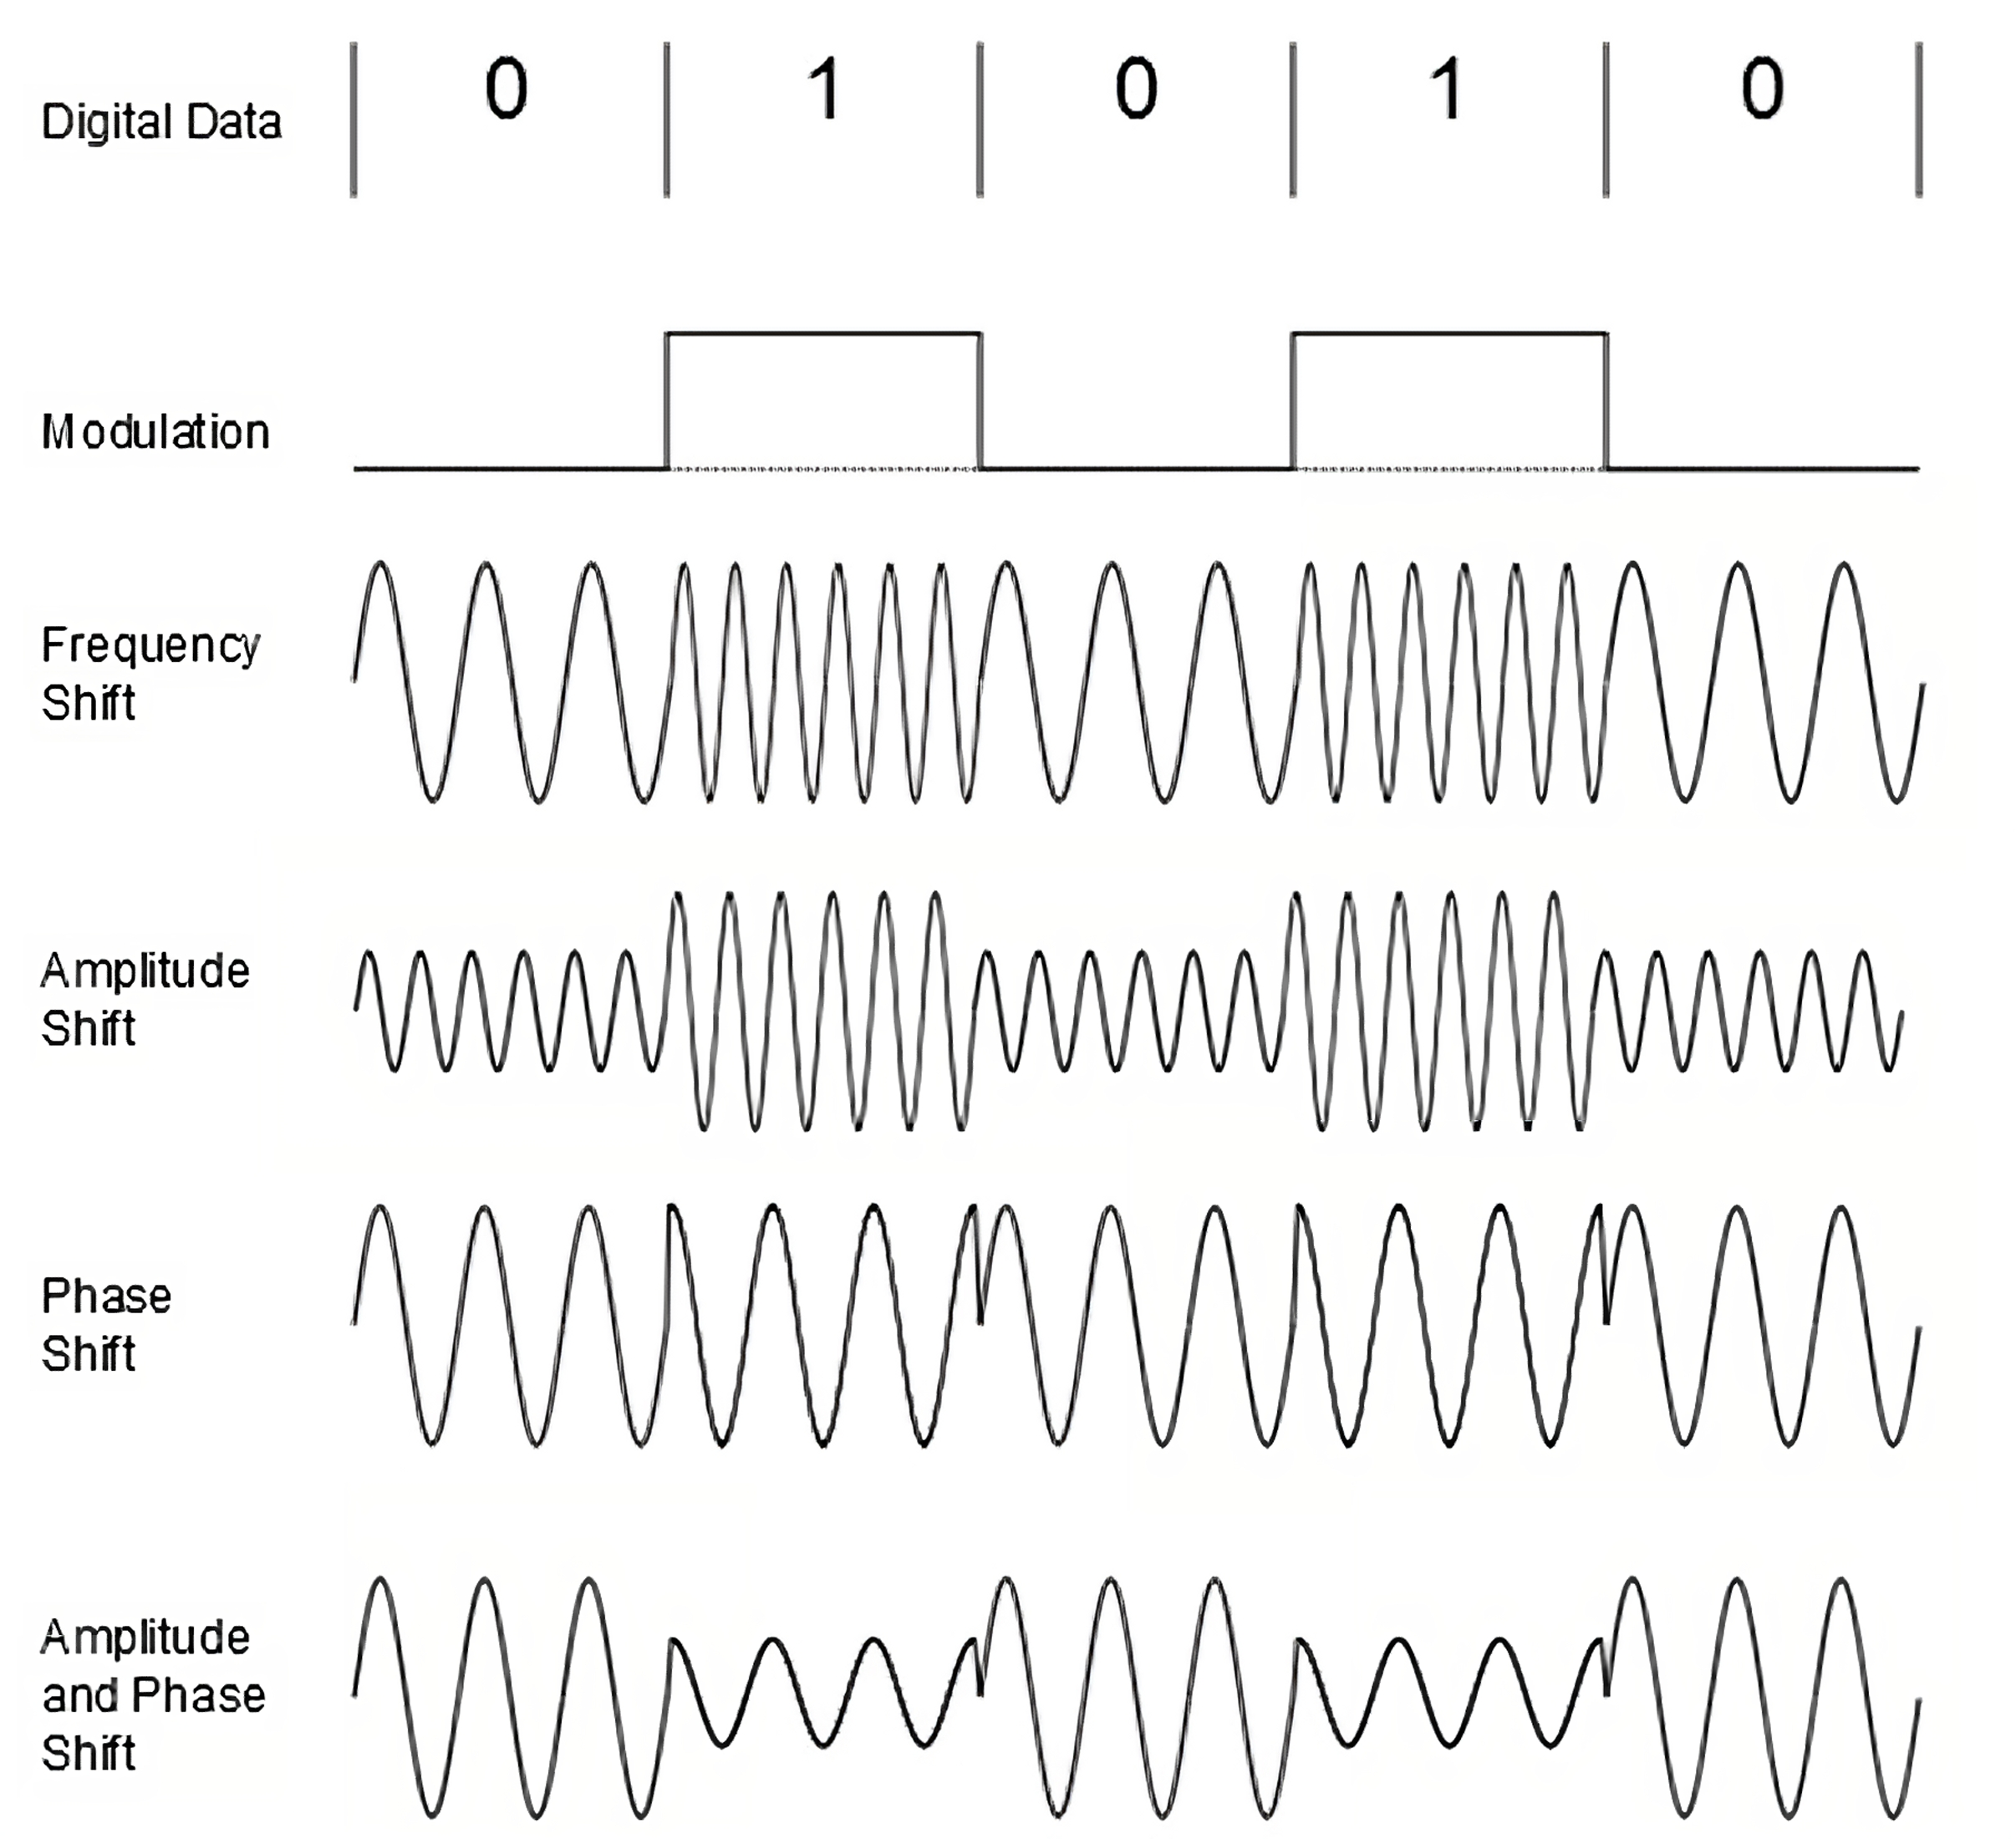
\includegraphics[width=0.8\linewidth]{modulations.png}
	\caption[Modulations]{Example of modulations Source: https://content.cdntwrk.com/ ref: URL06}
	\label{fig:modulations}
\end{figure}

Note that the \gls{gps} system uses \gls{bpsk} to transmit the \gls{ca} code.


\subsection{Channel access methods}

There exist different methods for multiple devices to communicate on a same transmission medium. Three of the popular methods are \gls{fdma}, \gls{tdma} and \gls{cdma}.

\begin{itemize}
	\item \gls{fdma} divides the available bandwidth into multiple frequency channels, this means each signal sends data on a different frequency.
	\item \gls{tdma} divides the available bandwidth into multiple time channels, this means that each user gets the full bandwidth for a short period of time.
	\item \gls{cdma} uses the exact same frequency at the exact same time, thus multiple transmitters can broadcast data at the same time and on the same frequency. The discrimination between the different signals is done using a unique code for each transmitter (Cross-Correlation ).
\end{itemize}


\begin{figure}[H]
	\centering
	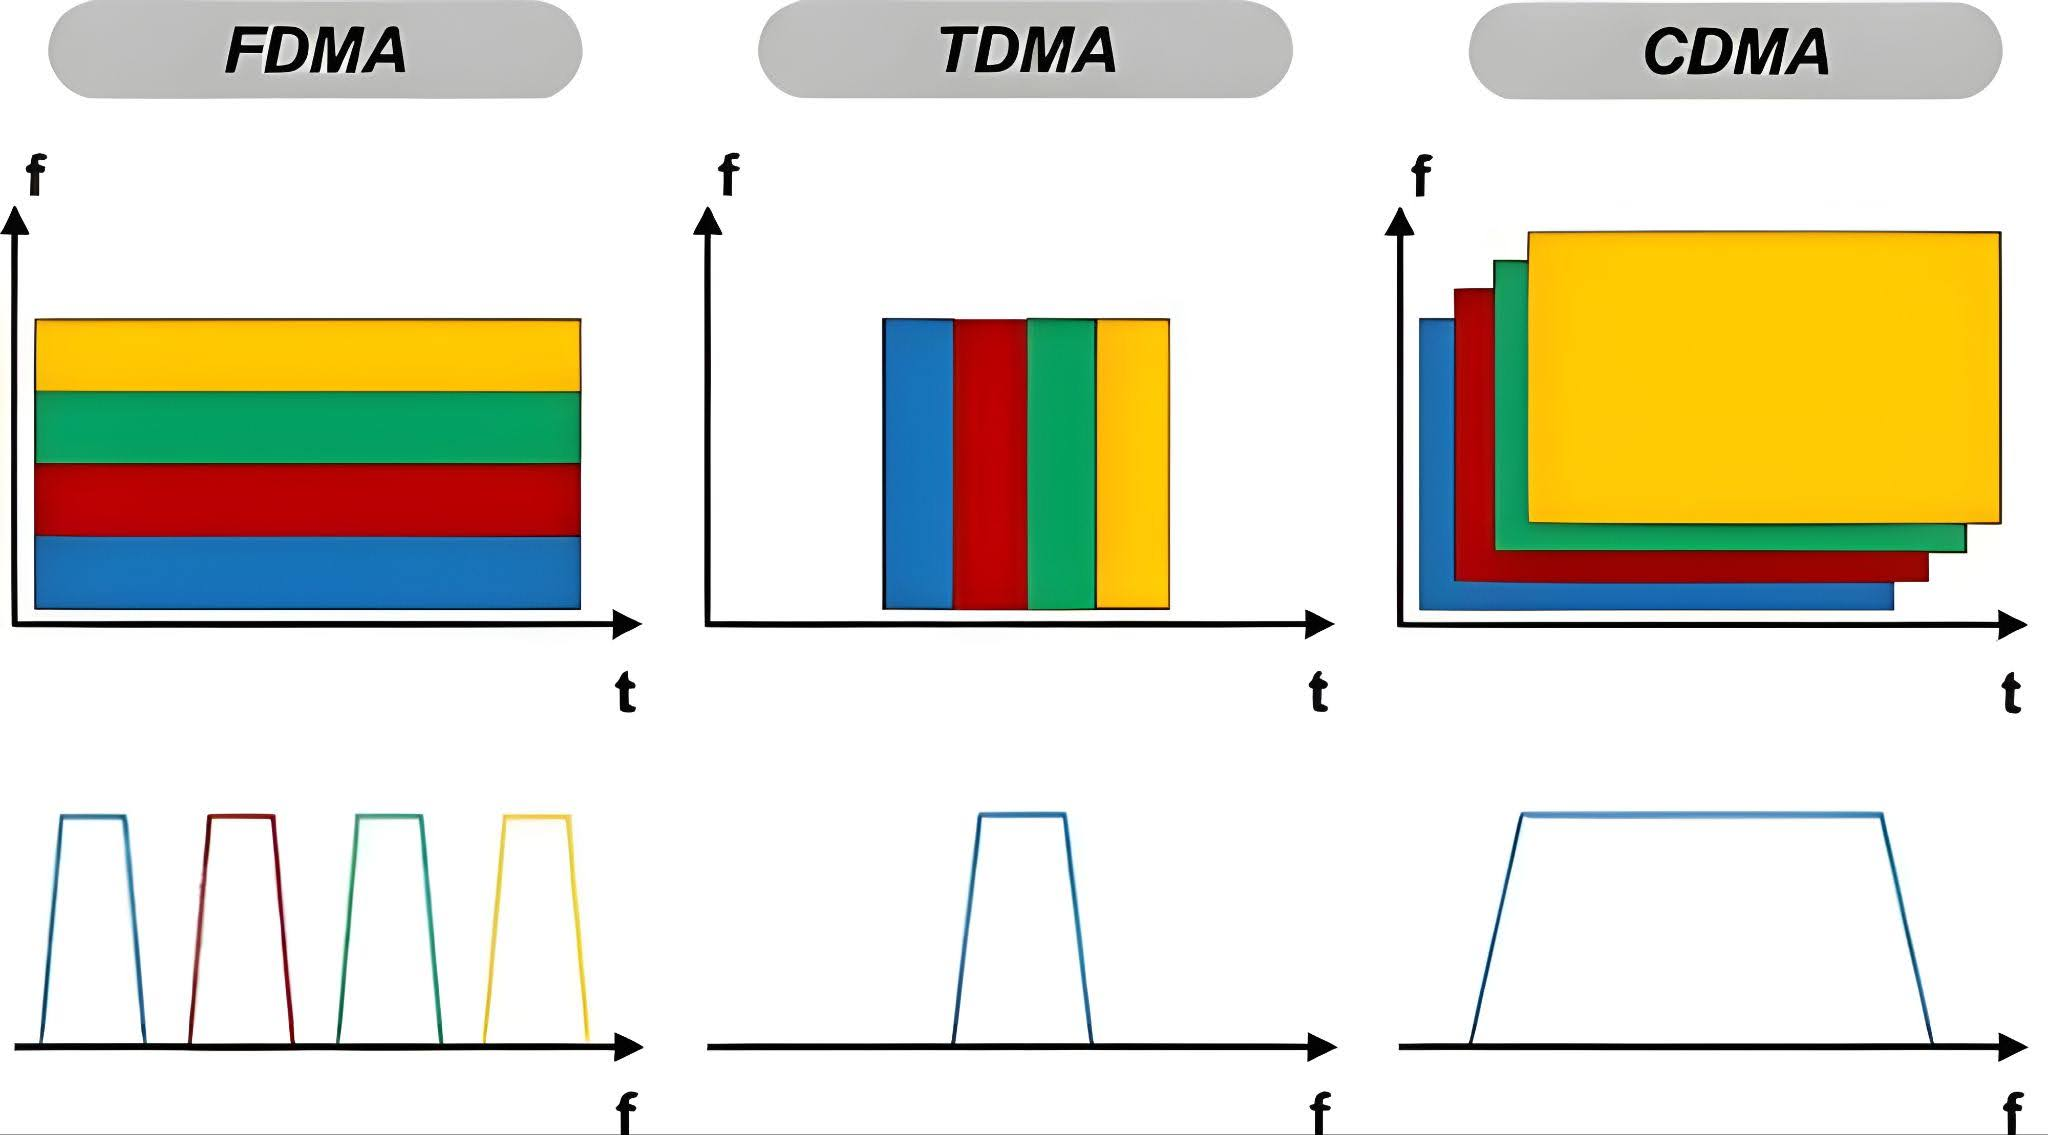
\includegraphics[width=0.8\linewidth]{cdma.jpg}
	\caption[Channel access methods]{Channel access methods visual description Source: https://www.researchgate.net/ ref: URL06}
	\label{fig:cdma}
\end{figure}

The \gls{gps} system uses \gls{cdma} to transmit the \gls{ca} code.

\section{Trilateration}

Trilateration is a method used to determine the position of an object using the geometry of the space. Often confused with \textbf{triangulation}, trilateration uses distances to determine the position of an object, while triangulation uses angles.

In order to get a position on a 2D plane, we need at least 3 distances from known points. In 3D, we need at least 4 distances from known points.

\begin{figure}[H]
	\centering
	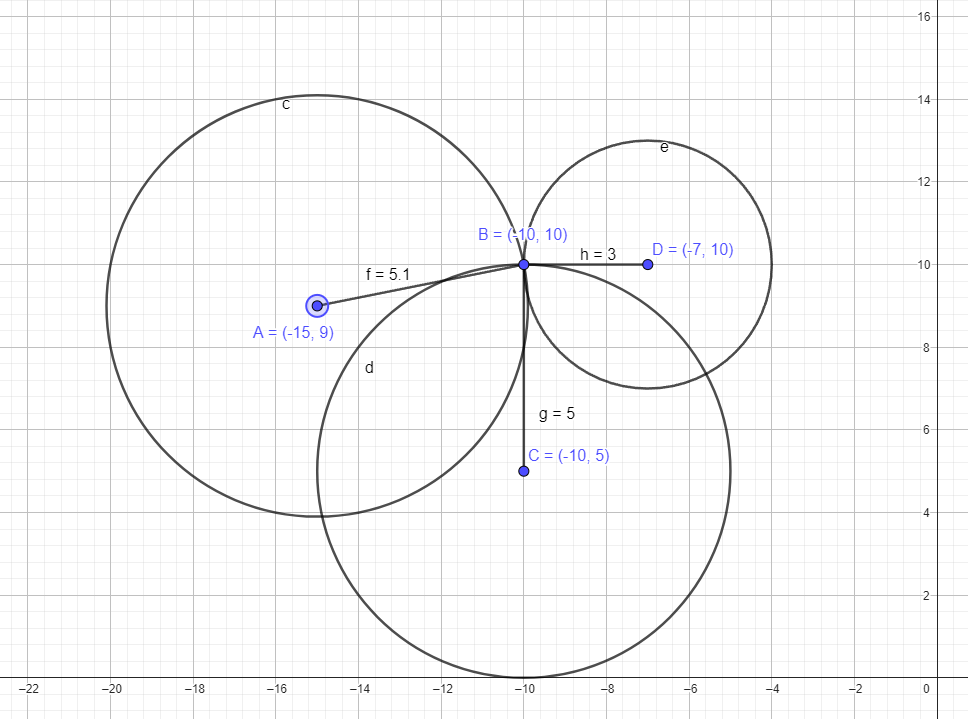
\includegraphics[width=0.8\linewidth]{trilateration.png}
	\caption[Trilateration example]{Trilateration example Source: Made by Jonas Stirnemann}
	\label{fig:trilateration_example}
\end{figure}

In this example, we have 3 known points \textit{A}, \textit{D} and \textit{C} and we know the distance from the unknown point to each of the known points \textit{f}, \textit{h} and \textit{g}. We can then calculate the position of the unknown point \textit{B} using the distances and the known positions of the other points.

\section{Software Defined Radio}

A \gls{sdr} is an hardware device that contains a fully fledged \gls{rf} frontend for modulating, creating and transmitting or receiving radio signals. These devices are designed to be connected to a computer via a fast interface like USB or Ethernet. The computer will then be a host multiple softwares that can generate or receive and process data via / from the \gls{sdr}.

These are very versatile devices that can be used for a wide range of applications like creating a simple FM radio receiver, a GSM base station, a GPS receiver or any simple or complex \gls{rf} based system.

We can observe an example block diagram of an \gls{sdr} in the next figure. It's composed of an USB port for communicating with the PC, an \gls{fpga} for processing the data and an \gls{rf} frontend for (de)modulating the signals and send/receive them through an antenna (usually SMA connector).

\begin{figure}[H]
	\centering
	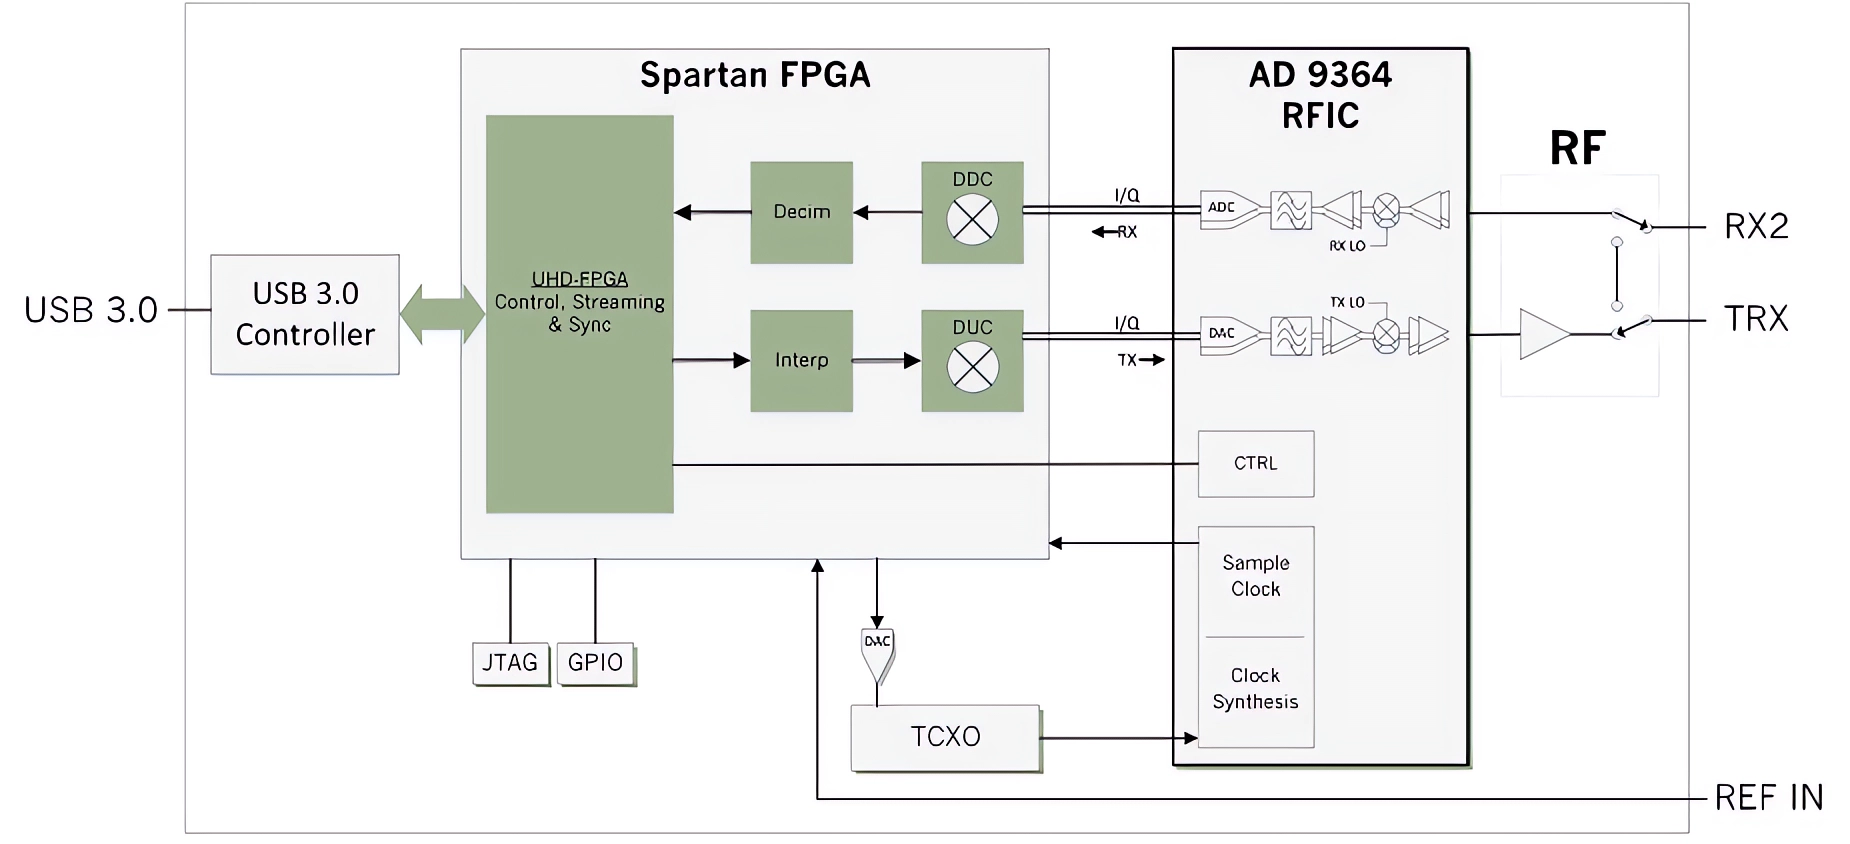
\includegraphics[width=1\linewidth]{sdr_schematics.png}
	\caption[Example block diagram of an SDR]{Example block diagram of an SDR Source: www.ettus.com ref : URL17}
	\label{fig:sdr_schematics}
\end{figure}



%\begin{minipage}{0.6\textwidth}
%	\begin{figure}[H]
%		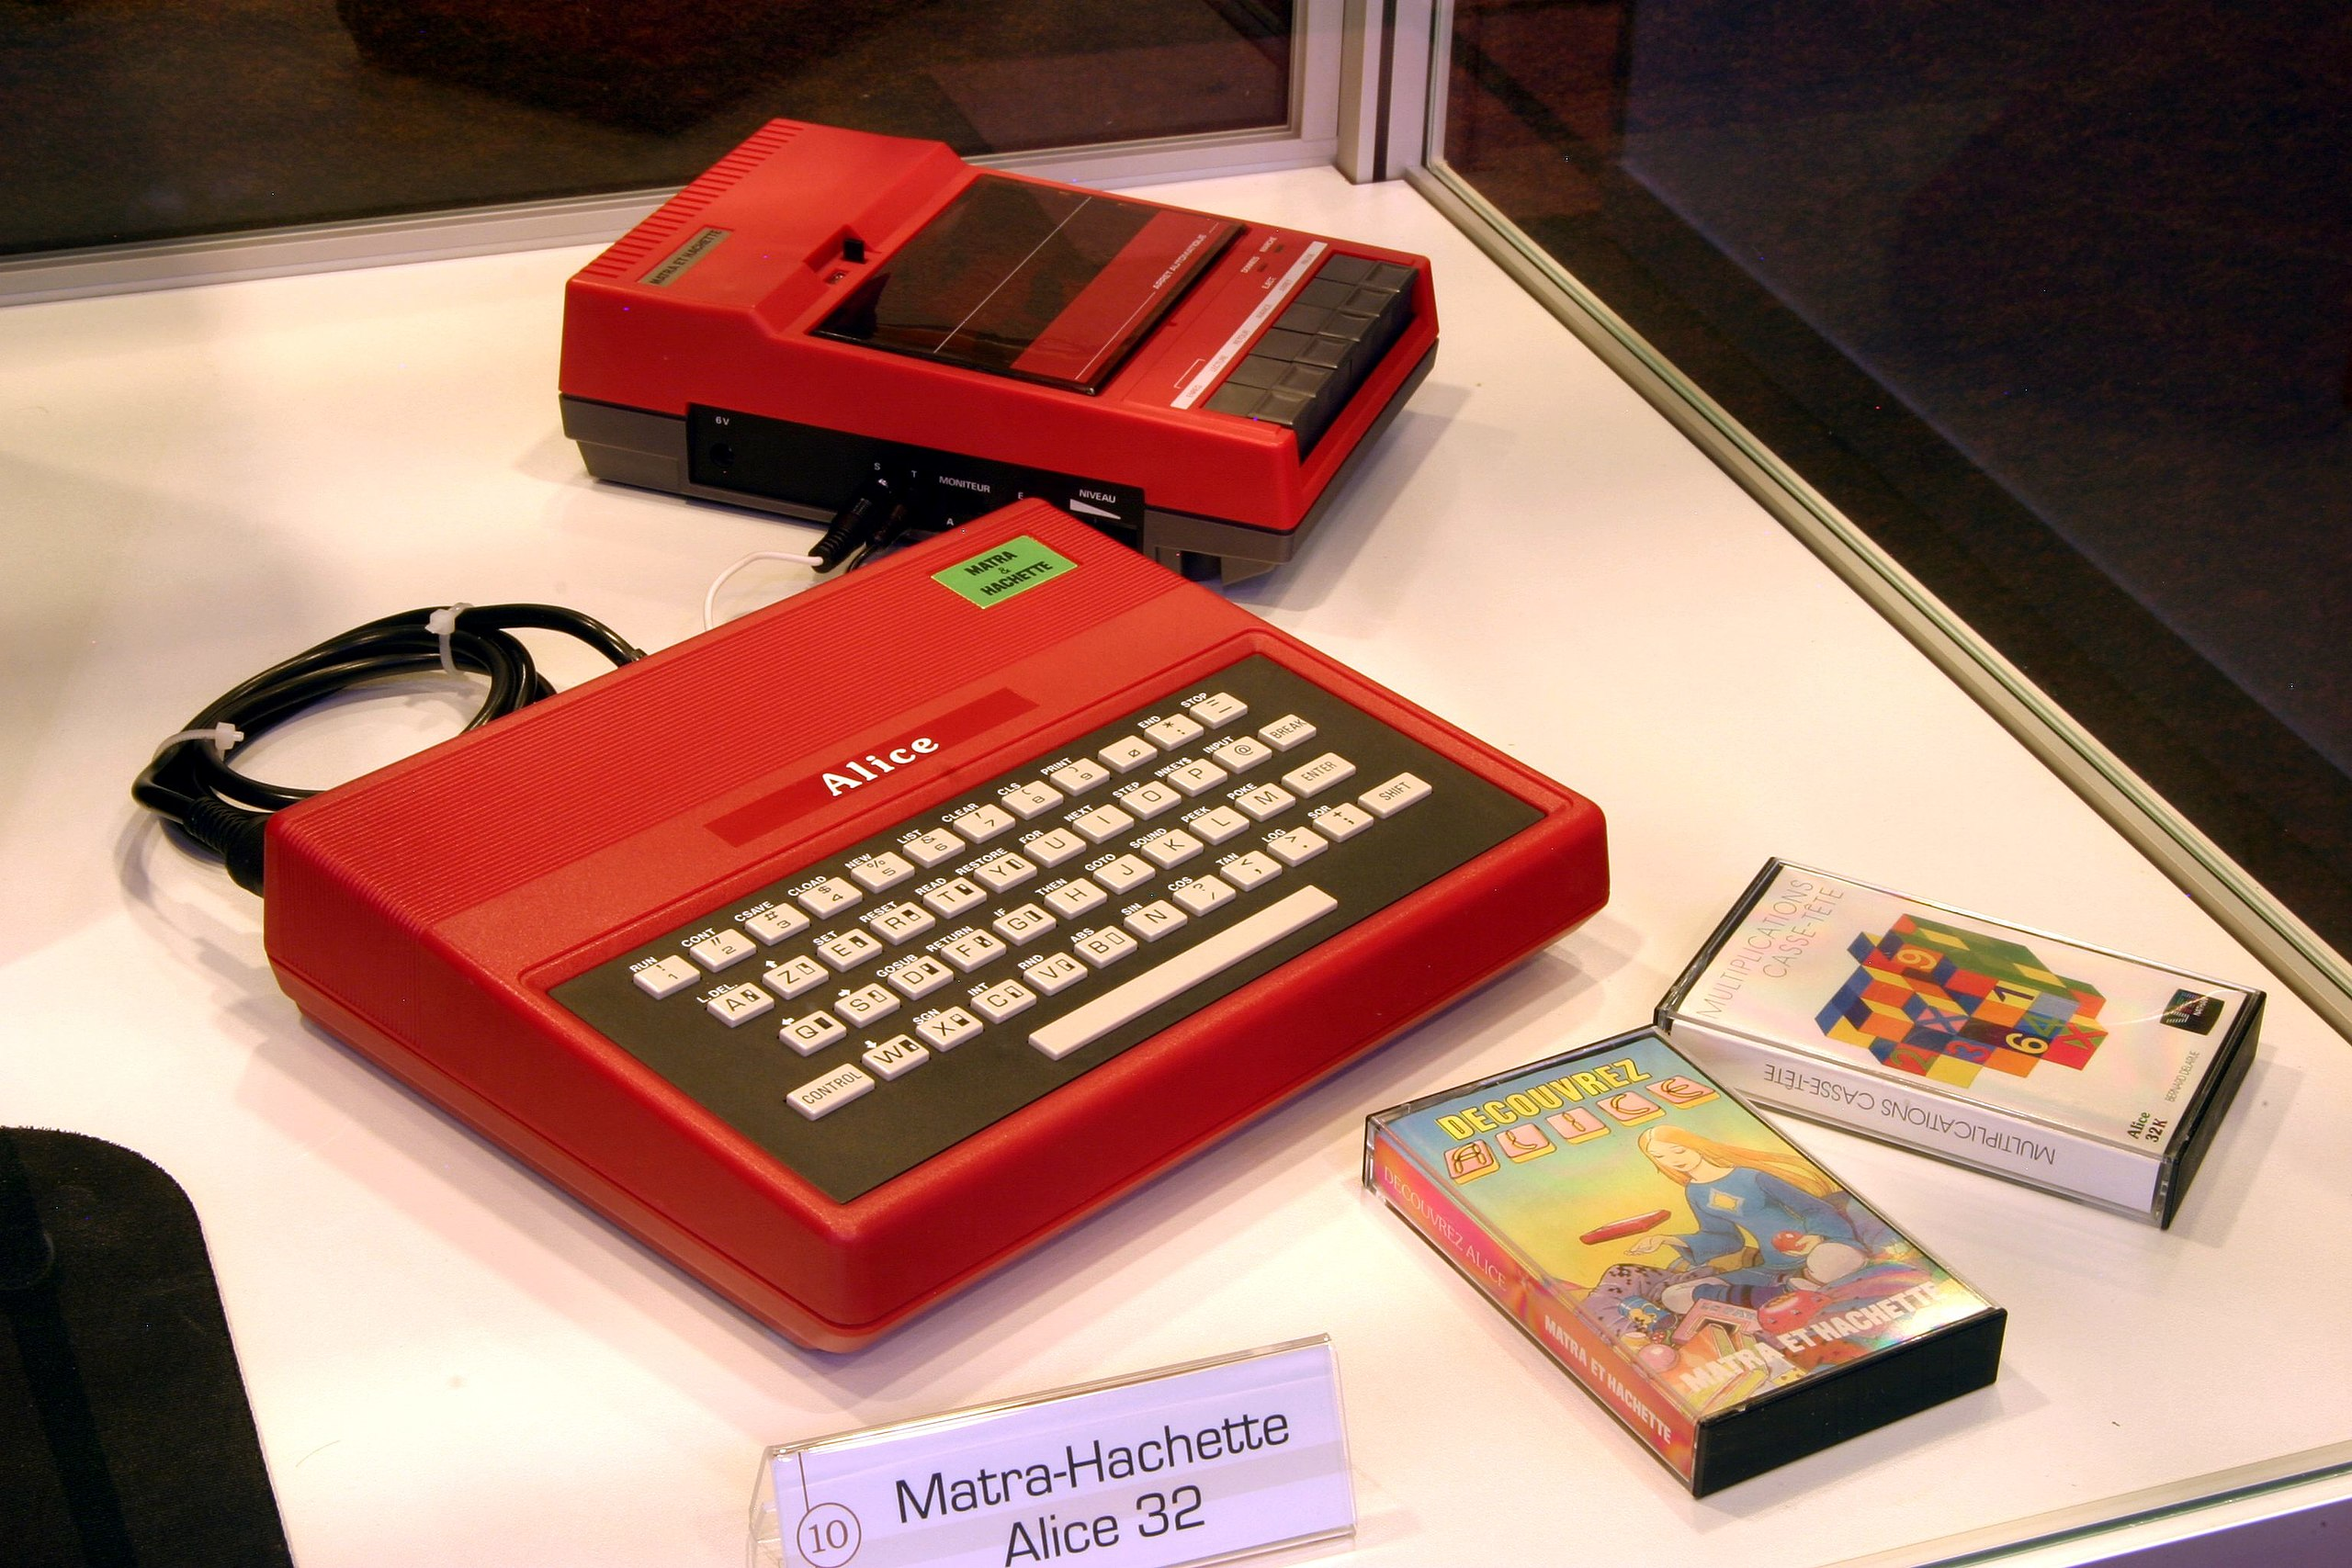
\includegraphics[width=\linewidth]{figures/ordi.jpg}
%		\caption{\label{fig:blue_rectangle} Rectangle}
%	\end{figure}
%\end{minipage} \hfill
%\begin{minipage}{0.2\textwidth}
%	Just some random text
%\end{minipage}

%\begin{figure}[tbph!]
%	\centering
%	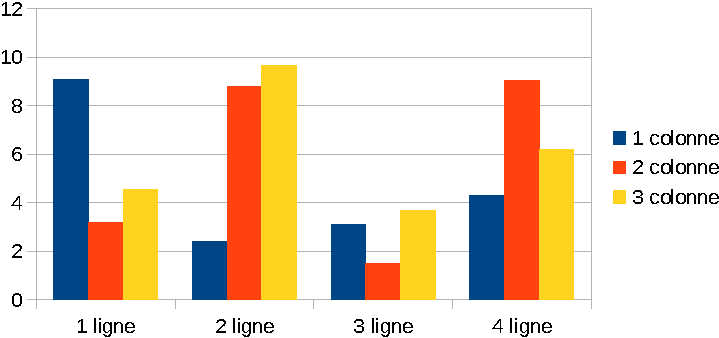
\includegraphics[width=0.7\linewidth]{chart}
%	\caption[Diagramme machin]{Diagramme machin. Source : tiré de Tartempion 2010, p. 42 / tiré de ce-site.ch, ref. URL01 / réalisé par Nom Prénom.}
%	\label{fig:chart1}
%\end{figure}


